\section{Results}

%Results:	control	input,	system	states,	comment	on	the	requirements,	and	comparisons	
%between	CompSOC and	MATLAB	outcomes
Figure \ref{fig:finalresult} shows the comparison of results in Simulink and CompSOC platform. While the simulation and experiment match for most parts, the minor deviations can be attributed to the exact delay differences between the platforms as discussed in \ref{sec:stad}. Then in Figure \ref{fig:Sresult} the derived values are displayed.
\begin{figure}[h]
	\begin{center}
		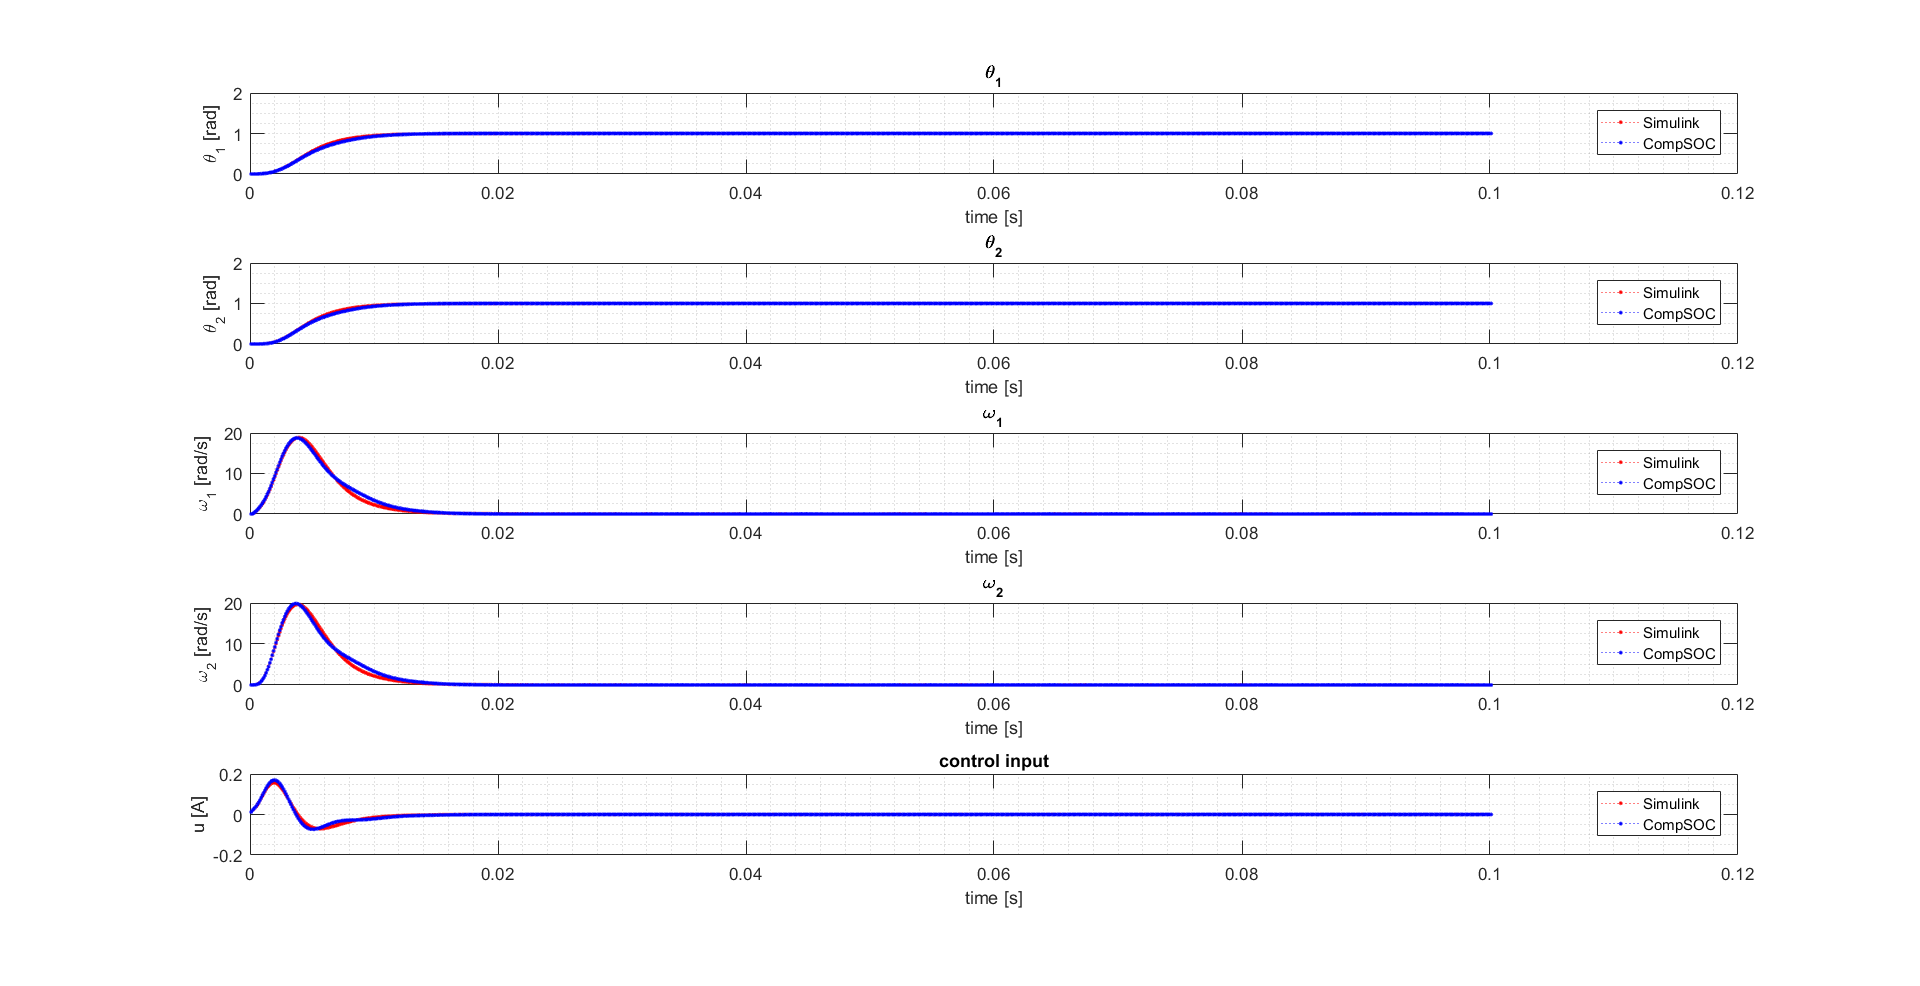
\includegraphics[width=\linewidth]{img/finalresult}
		\caption{Results comparison from Simulink and CompSOC.}
		\label{fig:finalresult}
	\end{center}
\end{figure}


\begin{figure}[h!]
	\begin{center}
		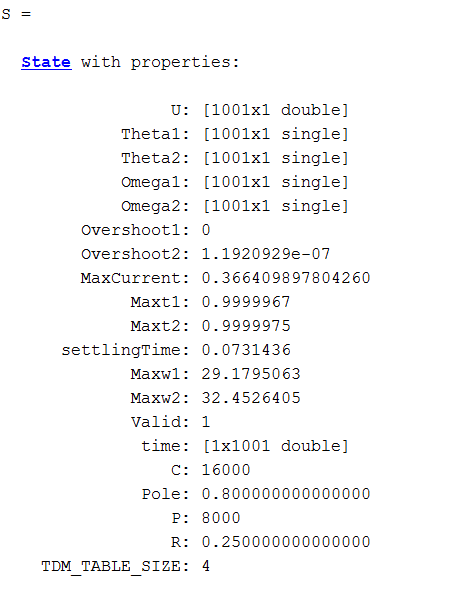
\includegraphics[width=0.5\linewidth]{img/S}
		\caption{Final values for the best solution found. All are well within required design parameters}
		\label{fig:Sresult}
	\end{center}
\end{figure}